
\chapter{Frameworks e linguaggi di programmazione utilizzati}

\section{Il linguaggio Python}

\begin{wrapfigure}[6]{l}{0.13\textwidth}  % Specifica la larghezza dell'immagine e il numero di righe da avvolgere
    \setlength{\fboxsep}{1pt} % Distanza tra l'immagine e il bordo
    \setlength{\fboxrule}{0pt} % Spessore del bordo
    \fbox{
\includegraphics[width=0.11\textwidth]{Immagini/Loghi/Python-logo.png}}  % Aggiungi il logo con contorno
\end{wrapfigure}

Per la realizzazione dei vari esperimenti e illustrazioni esposti nel corso della
tesi, è stato utilizzato il linguaggio di programmazione Python, un linguaggio di 
programmazione utilizzato per lo sviluppo dell’analisi empirica. 
Python è un linguaggio di programmazione ad alto livello noto per la 
sua: dinamicità, semplicità e flessibilità.
Esso è un linguaggio interpretato in grado di supportare paradigmi di 
programmazione come: la programmazione procedurale, la programmazione orientata agli 
oggetti e la programmazione funzionale.
Vanta la possibilità di interfacciarsi con diversi tipi di system call, librerie e 
sistemi a finestra ed è estensibile in C o C++. Può anche essere utilizzato come linguaggio di 
estensione per applicazioni che necessitano di un’interfaccia programmabile. Python è in 
grado di combinare un potenziale notevole ad una sintassi molto chiara e infine si tratta di 
un linguaggio portatile: funziona su molte varianti di Unix, su MacOS e su Windows 
La nascita del linguaggio è attribuibile a Guido van Rossum, programmatore 
olandese laureatosi all’Università di Amsterdam con un Master in Matematica ed 
Informatica e conosciuto come il Benevolent Dictator for Life di Python. 
Con il tempo, Python, è diventato uno tra i più utilizzati
linguaggi di programmazione per l'ambito della \textit{data science} e 
\textit{data analytics}, con la crescente diffusione di progetti legati al 
Machine learning, Cloud computing e Big data. Ciò grazie anche
alla vasta raccolta di librerie \cite{Python_Wikipedia}.

Per la realizzazione dei vari programmi, alcune delle principali librerie che sono 
state utilizzate sono: %l'analisi dei dati sono:
\begin{itemize}
    \item \textbf{Numpy}, una libreria che fornisce supporto per array multidimensionali e 
    funzioni matematiche ad alte prestazioni per operare su di esse. 
    È particolarmente utile per manipolare grandi quantità di dati numerici in 
    modo efficiente;

    \item \textbf{Matplotlib} è una libreria per la visualizzazione dei dati. Consente di 
    realizzare grafici a linee, istogrammi, scatter plot e altro ancora;
    
    \item \textbf{Seaborn} è una libreria basata su Matplotlib che offre un'interfaccia più 
    intuitiva per la realizzazione di grafici statisticamente informativi, come le heatmap e 
    le matrici di confusione. 
    
    \item \textbf{Scikit-learn} è una libreria per l'apprendimento automatico. Fornisce una 
    vasta raccolta di strumenti per la classificazione, la regressione e il 
    clustering;

    \item \textbf{Pandas} è una libreria progettata per la manipolazione e l'analisi dei dati strutturati;
 
    \item \textbf{Pytorch} è una libreria open-source per l'apprendimento automatico e 
    il deep learning. Fornisce strumenti per creare reti neurali e algoritmi di 
    apprendimento basati su tensori.
\end{itemize}



\section{Frameworks per lo sviluppo di reti neurali}
Le reti neurali artificiali hanno dimostrato di essere all'avanguardia 
in molti casi di apprendimento supervisionato, ma programmare manualmente 
una rete neurale può essere un compito impegnativo. 
% Di conseguenza, sono stati 
% creati framework come TensorFlow e PyTorch per semplificare la creazione, 
% il servizio e la scalabilità dei modelli di deep learning.
Con l'aumento dell'interesse per il deep learning negli ultimi anni, 
si è assistito a un'esplosione di strumenti di apprendimento automatico. 
Negli ultimi anni sono stati introdotti e sviluppati a ritmo sostenuto 
framework di deep learning come PyTorch, TensorFlow, Keras, Chainer e altri.

\begin{figure}[H]
    \centering
    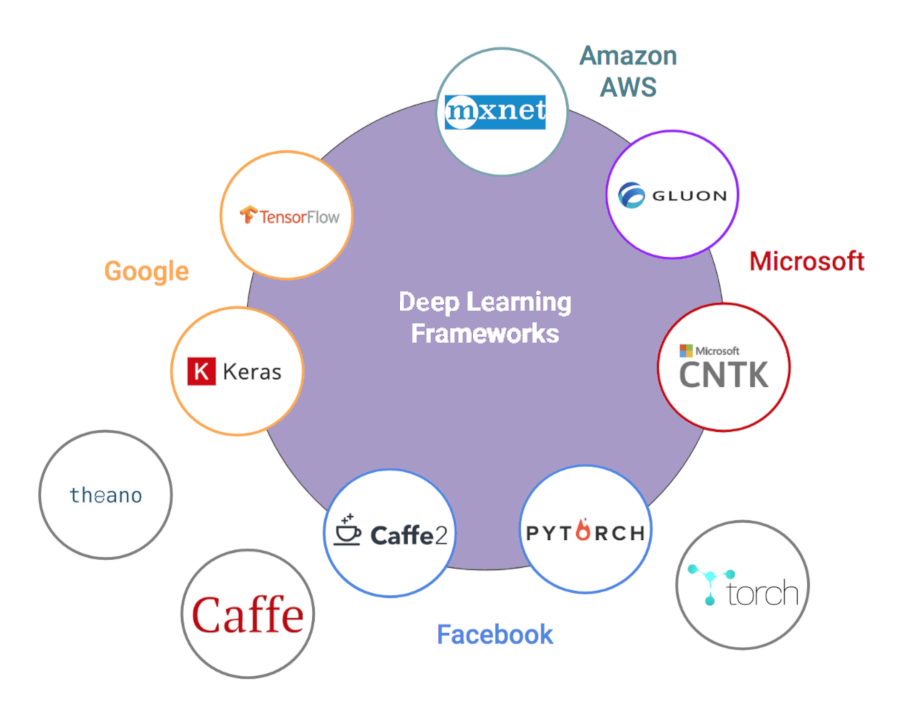
\includegraphics[width=0.55\textwidth]{Immagini/Generiche/Deep Learning Frameworks.png}
    \caption{Alcuni dei principali framework \cite{Framework_Devopedia}.}
\end{figure}

Questi framework forniscono unità di rete neurale, funzioni di costo e 
ottimizzatori per assemblare e addestrare modelli di rete neurale, permettendo di
semplificare e velocizzare lo sviluppo di questi modelli.
Alcuni di questi frameworks come Tensorflow, PyTorch e Keras; Sono disponibili
per il linguaggio di programmazione Python, sotto forma di libreria, fornendo un
API per la progettazione e l’addestramento di modelli.  


\subsection{Trends dei frameworks}

\begin{figure}[H]
    \centering
    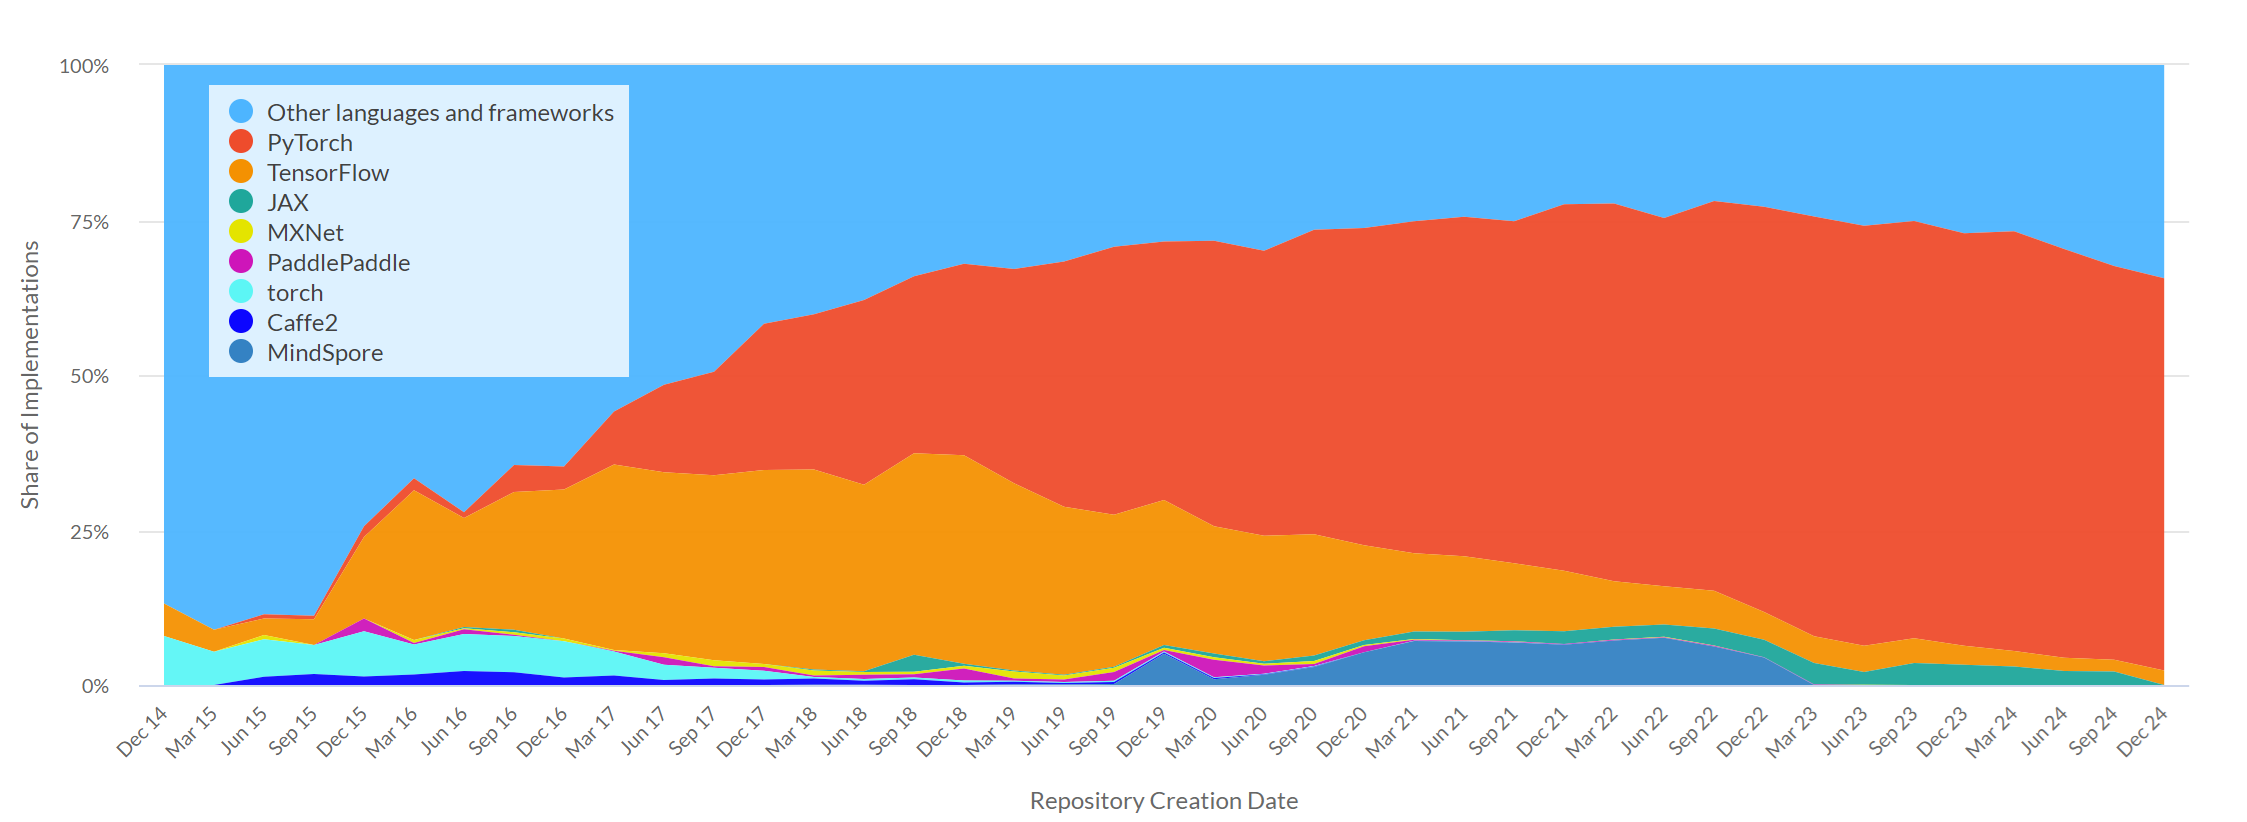
\includegraphics[width=1.0\textwidth]{Immagini/Grafici/graficoFrameWork.png}
    \caption{Trends dei frameworks \cite{Framework_PapersWithCode}.}
\end{figure}

Il grafico mostra l'andamento dei framework utilizzati nei repository GitHub 
dedicati alle implementazioni di articoli scientifici.
L'asse temporale indica la data di creazione dei repository, consentendo di 
osservare come la popolarità dei vari framework sia cambiata nel tempo.
Tra i più utilizzati spiccano TensorFlow e PyTorch, due strumenti fondamentali e 
molto apprezzati nel campo dell'apprendimento automatico.
Pertanto, per la realizzazione delle reti neurali, utilizzeremo Pytorch, in quanto è uno 
dei migliori framework per chi si avvicina per la prima volta a questo ambito. 



\subsection{TensorFlow}
% TensorFlow wrapfigure
\begin{wrapfigure}[6]{l}{0.25\textwidth}  % Specifica la larghezza dell'immagine e il numero di righe da avvolgere
    \setlength{\fboxsep}{1pt} % Distanza tra l'immagine e il bordo
    \setlength{\fboxrule}{0pt} % Spessore del bordo
    \fbox{
\includegraphics[width=0.23\textwidth]{Immagini/Loghi/Tensorflow_v2.png}}  % Aggiungi il logo con contorno
\end{wrapfigure}

Tensorflow \cite{Framework_AnalyticsVidhya,Framework_VisoAI,Framework_Devopedia} è una libreria open source sviluppata da Google che fornisce risorse per la creazione di modelli per l’apprendimento automatico.  
Rilasciata ufficialmente nel 2015, è diventata velocemente una delle più popolari soprattutto grazie 
al supporto per diversi linguaggi di programmazione, come Python, C++ e R.
In oltre dispone di un'ottima documentazione e linee guida,che la rendono un’ottima scelta per chi si avvicina per la prima volta a tale mondo.  

Tra i principali vantaggi, TensorFlow offre:
\begin{itemize}
    \item Supporto per l’esecuzione su GPU e TPU, che permette di accelerare i tempi di addestramento.
    \item Un ecosistema completo, che include TensorBoard per la visualizzazione e TensorFlow Lite per l’ottimizzazione su dispositivi mobili.
\end{itemize}
\aftergroup
\par
\subsection{Keras}
% Keras wrapfigure
\begin{wrapfigure}[4]{l}{0.25\textwidth}  % Specifica la larghezza dell'immagine e il numero di righe da avvolgere
    \setlength{\fboxsep}{2pt} % Distanza tra l'immagine e il bordo
    \setlength{\fboxrule}{0pt} % Spessore del bordo
    \fbox{
\includegraphics[width=0.22\textwidth]{Immagini/Loghi/Kerass.png}}  % Aggiungi il logo con contorno
\end{wrapfigure}

Keras \cite{Framework_AnalyticsVidhya,Framework_VisoAI,Framework_Devopedia} è 
una libreria open source scritta in Python e può essere eseguita su 
TensorFlow (oltre che su CNTK e Theano). L'interfaccia di TensorFlow può essere un 
po' ostica, poiché si tratta di una libreria di basso livello e i nuovi utenti 
potrebbero avere difficoltà a comprendere alcune implementazioni.
Keras, invece, è un'API di alto livello, sviluppata con l'obiettivo di consentire 
una sperimentazione rapida. Quindi, se si vogliono ottenere risultati rapidi, 
Keras si occuperà automaticamente dei compiti principali e genererà l'output.

\aftergroup
\par

\subsection{Pytorch}
% PyTorch wrapfigure
\begin{wrapfigure}[4]{l}{0.28\textwidth}  % Specifica la larghezza dell'immagine e il numero di righe da avvolgere
    \setlength{\fboxsep}{2pt} % Distanza tra l'immagine e il bordo
    \setlength{\fboxrule}{0pt} % Spessore del bordo
    \fbox{
\includegraphics[width=0.25\textwidth]{Immagini/Loghi/PyTorch_logo_black.png}}  % Aggiungi il logo con contorno
\end{wrapfigure}

PyTorch \cite{Framework_AnalyticsVidhya,Framework_VisoAI,Framework_Devopedia} è una libreria open source sviluppata da Facebook e introdotta per la 
prima volta nel 2016. Questa libreria è particolarmente apprezzata per la 
sua flessibilità con un'attenta considerazione delle prestazioni e per l'approccio 
dinamico al calcolo dei grafi computazionali. Oggi, la maggior parte del suo nucleo è scritto in C++, uno dei motivi principali 
per cui PyTorch può ottenere un overhead molto più basso rispetto ad 
altri framework. Ad oggi, PyTorch sembra essere il più adatto a ridurre 
drasticamente il ciclo di progettazione, addestramento e test di nuove reti 
neurali per scopi specifici. Per questo è diventato molto popolare nelle comunità 
di ricerca.

\subsection{PyTorch Lightning}

\begin{wrapfigure}[4]{l}{0.30\textwidth}  % Specifica la larghezza dell'immagine e il numero di righe da avvolgere
    \setlength{\fboxsep}{2pt} % Distanza tra l'immagine e il bordo
    \setlength{\fboxrule}{0pt} % Spessore del bordo
    \fbox{
\includegraphics[width=0.28\textwidth]{Immagini/Loghi/Lightning_Logo.png}}  % Aggiungi il logo con contorno
\end{wrapfigure}

PyTorch Lightning \cite{PyTorchLightning, PyTorchLightning_site} è una libreria Python 
open-source che fornisce un'interfaccia di 
alto livello per PyTorch. È un framework leggero e ad alte prestazioni che 
organizza il codice PyTorch per disaccoppiare la ricerca dall'ingegneria, rendendo 
così gli esperimenti di deep learning più facili da leggere e riprodurre,
accelerando così i tempi di sviluppo dei modelli. 
È stato progettato per creare modelli scalabili di deep learning che possono 
essere facilmente eseguiti su hardware distribuito.
In oltre, PyTorch Lightning possiede una struttura modulare che semplifica 
la gestione di training, validazione e logging.
\aftergroup
\par